% TA-IND-01: informe de análisis crítico de NATS JetStream.
% Compilar desde la carpeta informe/: pdflatex informe.tex; biber informe; pdflatex informe.tex; pdflatex informe.tex
\documentclass[12pt,a4paper]{article}
\usepackage[utf8]{inputenc}
\usepackage[T1]{fontenc}
\usepackage[spanish,es-tabla]{babel}
\usepackage{lmodern}
\usepackage{microtype}
\usepackage[a4paper,left=2.8cm,right=2.6cm,top=2.7cm,bottom=2.6cm]{geometry}
\usepackage{graphicx}
\usepackage{float}
\usepackage{booktabs}
\usepackage{longtable}
\usepackage{array}
\usepackage{setspace}
\usepackage{xurl}
\usepackage{csquotes}
\usepackage[hidelinks]{hyperref}
\usepackage{fancyhdr}
\usepackage[backend=biber,style=ieee,sorting=none]{biblatex}
\addbibresource{../referencias.bib}
\graphicspath{{../imagenes/}{../diagramas/}{../experimentos/capturas/}{../Anexos/}{../Anexos/fuentes/}{../anexos/}{../anexos/fuentes/}}
\setstretch{1.24}
\setlength{\parindent}{1.1cm}
\setlength{\parskip}{0.12em}
\pagestyle{fancy}
\fancyhf{}
\fancyhead[L]{\footnotesize TA-IND-01 -- Aplicaciones Distribuidas}
\fancyhead[R]{\footnotesize NATS JetStream}
\fancyfoot[C]{\thepage}
\renewcommand{\headrulewidth}{0.35pt}
\setlength{\headheight}{15pt}


\begin{document}
\pagenumbering{gobble}

% CARÁTULA: datos tomados de la portada facilitada para esta actividad.
\begin{titlepage}
  \centering
  \vspace*{0.15cm}
  
\includegraphics[height=3.5cm]{logo-uteq.jpg}\par
  \vspace{0.65cm}
  {\Large\bfseries UNIVERSIDAD TÉCNICA ESTATAL DE\\QUEVEDO\par}
  \vspace{0.5cm}
  {\large\bfseries Facultad de Ciencias de la Computación\par}
  {\large Carrera de Software\par}
  \vspace{0.72cm}
  {\normalsize\bfseries Asignatura\par}
  {\normalsize Aplicaciones Distribuidas\par}
  \vspace{0.44cm}
  {\normalsize\bfseries Actividad\par}
  {\normalsize TA-IND-01 -- Informe Académico Individual\\Análisis Crítico de Sistemas Distribuidos (Unidad 1)\par}
  \vspace{0.24cm}
  {\small\itshape Análisis de NATS JetStream y comparación con Apache Pulsar\par}
  \vspace{0.48cm}
  {\normalsize\bfseries Docente\par}
  {\normalsize Ing. Gleiston Cicerón Guerrero Ulloa\par}
  \vspace{0.38cm}
  {\normalsize\bfseries Estudiante\par}
  {\normalsize Quintero Rico Luis David\par}
  \vspace{0.38cm}
  {\normalsize\bfseries Curso\par}
  {\normalsize Séptimo nivel, paralelo B\par}
  \vspace{0.38cm}
  {\normalsize\bfseries Repositorio\par}
  {\footnotesize\url{https://github.com/Kinetro/TA-IND-01-Unidad1.git}\par}
  \vfill
  {\normalsize\bfseries Año lectivo 2026--2027\par}
  {\normalsize Quevedo -- Los Ríos -- Ecuador\par}
  {\normalsize 15 de noviembre de 2026\par}
\end{titlepage}

\clearpage
\pagenumbering{arabic}
\section*{Resumen}
\addcontentsline{toc}{section}{Resumen}
Este informe examina la arquitectura distribuida de NATS JetStream y su comportamiento ante la caída controlada de un servidor, tomando Apache Pulsar como sistema de comparación. Se estudian los componentes que intervienen en la publicación, persistencia y recuperación de mensajes, así como la coordinación entre réplicas. Para comprobar el funcionamiento se configuró en CachyOS un clúster local de tres nodos y un flujo denominado \texttt{PRUEBA\_R3}, con tres réplicas. Primero se almacenaron y recuperaron tres mensajes. Luego se detuvo el nodo líder y se observó la elección de otro líder; durante la interrupción se pudo incorporar un cuarto mensaje. Finalmente, el servidor detenido se reinició y volvió a aparecer sincronizado, conservándose los cuatro mensajes. La prueba respalda la capacidad del clúster para tolerar la pérdida de uno de sus tres nodos mientras mantiene el quórum, pero no constituye una medición de latencia ni una simulación de partición de red. El análisis se apoya en documentación técnica y artículos científicos para distinguir los resultados observados de las propiedades generales del sistema.

\section{Introducción}
Los sistemas que intercambian eventos entre aplicaciones necesitan enviar mensajes sin obligar al emisor y al receptor a estar conectados al mismo tiempo. Esta necesidad aparece en servicios web, procesos empresariales, sistemas de monitoreo y aplicaciones que generan datos continuamente. NATS emplea el modelo de publicación y suscripción: un emisor publica en un \emph{subject} y los receptores interesados pueden recibir ese mensaje. Sin embargo, en el servicio básico de NATS la entrega no implica almacenamiento para una lectura posterior. JetStream añade flujos persistentes (\emph{streams}) y mecanismos de lectura y confirmación, de modo que los mensajes pueden conservarse y recuperarse después \cite{natsjetstream}.

Cuando el servicio de mensajería depende de una sola máquina, la caída de ese servidor puede interrumpir el acceso a la información. NATS JetStream permite configurar varias réplicas del mismo flujo y coordinarlas mediante consenso Raft. Este diseño permite examinar una decisión importante de los sistemas distribuidos: la necesidad de mantener acuerdos entre nodos para confirmar escrituras, sin asumir que todos estarán siempre disponibles \cite{natsclustering}.

Una aplicación documentada por Ju, Seo y Kim utiliza NATS JetStream como base de un bus de eventos para compartir información entre clústeres. Ese caso permite ilustrar su uso fuera de una prueba de laboratorio, aunque estudia una plataforma IoT completa y no reproduce nuestro experimento de fallos \cite{ju2026}.

Se eligió JetStream porque se puede ejecutar y observar directamente desde una computadora con CachyOS. Para este trabajo se configuraron tres procesos locales y un flujo replicado; por tanto, los resultados describen este entorno de prueba y no una instalación geográficamente distribuida ni una evaluación de rendimiento a gran escala. Como referencia de otro enfoque se utiliza Apache Pulsar, cuya arquitectura separa los servidores que atienden a los clientes del almacenamiento persistente gestionado por Apache BookKeeper \cite{pulsararchitecture}. La revisión de Do y colaboradores describe en Pulsar multitenencia, replicación geográfica y separación del plano de almacenamiento, características que ayudan a explicar su diseño \cite{do2025}. Dyjach y Plechawska-Wójcik evaluaron Pulsar frente a Kafka y RabbitMQ bajo escenarios de rendimiento concretos; ese trabajo no incluyó a NATS JetStream y sus resultados no constituyen una comparación directa entre los dos sistemas elegidos \cite{dyjach2024}. La comparación del presente informe se centrará, por tanto, en la arquitectura y las garantías de operación documentadas.

\section{Arquitectura de NATS JetStream}
NATS JetStream funciona sobre servidores NATS que reciben publicaciones de los clientes y almacenan los mensajes correspondientes a un flujo. Un \emph{stream} se asocia a uno o varios patrones de asuntos (\emph{subjects}); al llegar una publicación que coincide con el patrón, JetStream puede almacenar ese mensaje en el flujo. JetStream también dispone de consumidores persistentes o temporales que gestionan el avance de la lectura y las confirmaciones de entrega \cite{natsjetstream}. En esta práctica la recuperación puntual de mensajes se verificó mediante el comando \texttt{nats stream get}, que consulta directamente el contenido almacenado y no equivale a crear un consumidor duradero.

\subsection{Configuración implementada}
Se ejecutaron tres instancias de \texttt{nats-server} en la misma computadora. Cada proceso utilizó un directorio de almacenamiento independiente y dos puertos: uno para las conexiones de clientes y otro para las rutas entre servidores.

\begin{table}[H]
\centering
\caption{Configuración local de los nodos NATS JetStream.}
\begin{tabular}{@{}llll@{}}
\toprule
Servidor & Puerto de cliente & Puerto de clúster & Almacenamiento \\ \midrule
\texttt{nodo1} & 4222 & 6222 & \texttt{datos/nodo1} \\
\texttt{nodo2} & 4223 & 6223 & \texttt{datos/nodo2} \\
\texttt{nodo3} & 4224 & 6224 & \texttt{datos/nodo3} \\ \bottomrule
\end{tabular}
\label{tab:nodos}
\end{table}

Los nodos se enlazaron por rutas locales dentro del clúster \texttt{laboratorio}. Se creó el flujo \texttt{PRUEBA\_R3}, asociado al patrón \texttt{replica.>}, con almacenamiento en archivos y factor de replicación tres. En esta configuración cada réplica mantiene una copia del estado del flujo; un líder coordina las escrituras y se requiere la mayoría de dos de tres nodos para alcanzar el quórum de consenso \cite{natsclustering}.

\subsection{Relación con el experimento}
Antes del fallo, la consulta de estado mostró a \texttt{nodo3} como líder y a \texttt{nodo1} y \texttt{nodo2} como réplicas actualizadas. Tras detener \texttt{nodo3} mediante \texttt{Ctrl+C}, \texttt{nodo1} asumió el liderazgo y \texttt{nodo2} continuó sincronizado. Se almacenó un cuarto mensaje mientras el tercer nodo estaba fuera de servicio. Al reiniciarlo, el estado volvió a mostrar las tres réplicas actualizadas, y los cuatro mensajes permanecieron disponibles. Estas observaciones corresponden a una interrupción de proceso controlada, no a una partición de red.

El esquema inicial dibujado a mano identifica el publicador, el clúster, los tres nodos y el cliente lector. El diagrama definitivo de draw.io amplía ese bosquejo al especificar los puertos, las rutas entre servidores, el factor de replicación y los cambios de liderazgo observados. La versión PNG del diagrama se incorpora desde la carpeta \texttt{diagramas/}. Se trata del diseño utilizado para explicar la prueba; las flechas representan conexiones de cliente y rutas entre servidores, no una medición de los mensajes que circularon por cada enlace.

% Se utiliza el nombre real del archivo exportado desde draw.io en el repositorio.
% Si el PNG no existe, la compilacion falla explicitamente.
\IfFileExists{../diagramas/arquitectura_nats.drawio.png}{%
\begin{figure}[H]
\centering
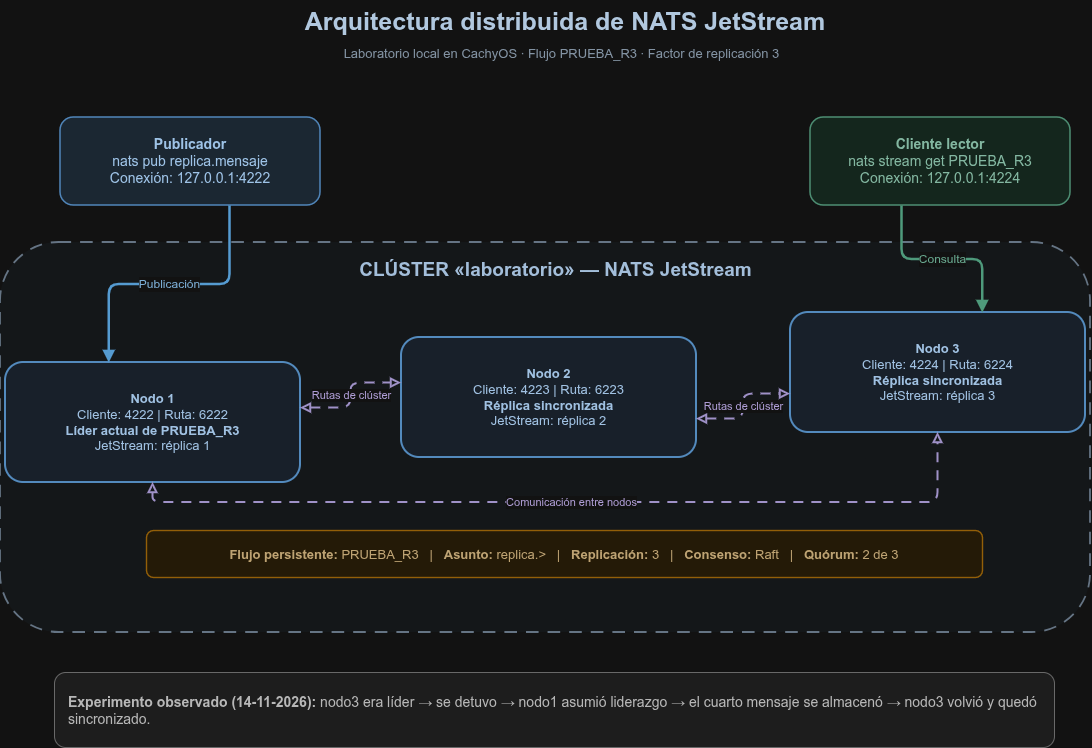
\includegraphics[width=0.98\linewidth,keepaspectratio]{arquitectura_nats.drawio.png}
\caption{Diagrama digital del clúster NATS JetStream.}
\label{fig:arquitectura}
\end{figure}
}{\PackageError{TA-IND-01}{Falta el diagrama PNG}{Se requiere diagramas/arquitectura_nats.drawio.png para compilar.}}


\section{Análisis con los conceptos de la Unidad 1}

\subsection{Transparencias de distribución}
La transparencia consiste en ocultar ciertos detalles de un sistema distribuido sin impedir que el usuario comprenda sus limitaciones. En NATS JetStream, la abstracción principal es el flujo de mensajes: una aplicación publica en un asunto y no necesita administrar manualmente las copias del flujo. Sin embargo, esto no significa que todas las formas de transparencia estén resueltas por completo \cite{natsjetstream,natsclustering}.

\begingroup
\small
\begin{longtable}{@{}p{2.8cm}p{2.4cm}p{7.9cm}@{}}
\caption{Evaluación de transparencias de distribución de NATS JetStream.}\label{tab:transparencias}\\
\toprule
\textbf{Transparencia} & \textbf{Grado} & \textbf{Análisis aplicado} \\ \midrule
Acceso & Alta & Se publica y consulta por asuntos y flujos, sin manejar directamente los archivos de almacenamiento de cada réplica. \\
Ubicación & Parcial & El cliente puede utilizar un servidor del clúster, que encamina solicitudes al líder; aun así, debe disponer de direcciones de conexión válidas. \\
Migración & Condicionada & Las réplicas pueden trasladarse a otros servidores mediante operaciones de administración; requiere un servidor de destino y no se probó. Cambiar de líder no migra una réplica. \\
Reubicación & No comprobada & NATS documenta el movimiento de réplicas durante el servicio. Esa operación depende del quórum y de servidores disponibles; aquí solo se observó un cambio de líder. \\
Replicación & Alta & La configuración del flujo indica tres réplicas y el sistema gestiona su coordinación; no garantiza que todas estén actualizadas exactamente al mismo instante. \\
Concurrencia & Parcial & Varios clientes pueden publicar o leer; el líder ordena las escrituras replicadas, pero las aplicaciones deben manejar confirmaciones y posibles reentregas. \\
Fallos & Parcial & Una réplica puede fallar y otra asumir el liderazgo si queda quórum. La pérdida de la mayoría o de los servidores físicos compartidos impide continuar. \\ \bottomrule
\end{longtable}
\endgroup

La prueba local permite observar principalmente la replicación y la tolerancia parcial a fallos: se mantuvo el nombre \texttt{PRUEBA\_R3} aunque el líder cambió de \texttt{nodo3} a \texttt{nodo1}. La reasignación de réplicas a otro servidor es una operación administrativa documentada, que no se probó porque nuestro laboratorio solo tenía tres servidores y no un destino adicional \cite{natspeers}. Un relevo de liderazgo no demuestra migración de datos ni reubicación física. Además, los tres procesos compartían el mismo equipo y, por tanto, un fallo completo del sistema operativo afectaría simultáneamente a todos.

\subsection{Teorema CAP y extensión PACELC}
El teorema CAP estudia qué ocurre cuando un sistema distribuido enfrenta una \emph{partición de red}: si dos grupos de nodos dejan de comunicarse, no es posible exigir a la vez que todos respondan correctamente y que todos mantengan una única visión consistente de las operaciones. En JetStream hay que distinguir el plano de mensajería de \emph{Core NATS} del flujo persistente replicado, porque sus garantías no son idénticas.

\paragraph{Durante una partición (CAP).}
Para un flujo JetStream con \(R=3\), el líder coordina las entradas de un registro Raft y una escritura debe alcanzar la mayoría de dos nodos para quedar confirmada. Si una partición separa a un servidor de los otros dos, el grupo mayoritario puede continuar confirmando escrituras; la parte aislada no puede hacerlo sin quórum. En ese sentido, el \emph{flujo replicado} prioriza la consistencia de las escrituras confirmadas sobre la disponibilidad universal durante la partición, una orientación de tipo CP para esa operación, no una clasificación absoluta de todo NATS \cite{natsreplication}. Los lectores conectados a una réplica seguidora pueden observar un estado momentáneamente atrasado; por eso no debe interpretarse CP como sincronización instantánea de todas las lecturas.

La orientación CAP anterior se fundamenta en la documentación de NATS; la prueba local mostró continuidad con un nodo detenido, no una partición de red.

\paragraph{Sin partición (PACELC).}
PACELC añade una segunda decisión: cuando la red funciona normalmente, ¿qué compromiso existe entre latencia (L) y consistencia (C)? En JetStream, una publicación que solicita confirmación de almacenamiento mediante \emph{JetStream PubAck} espera la aprobación del quórum, lo que introduce coordinación entre servidores frente a una entrega sin persistencia. No necesita esperar a que las tres réplicas apliquen cada operación: con tres nodos basta el líder y un seguidor para confirmar la entrada \cite{natsreplication}. Esta elección favorece el orden y la confirmación replicada, con un coste de comunicación y latencia. Por otro lado, las lecturas directas de seguidores pueden ir retrasadas; no existe una única etiqueta PACELC rigurosa para todas las operaciones y configuraciones del producto.

También hay un compromiso de \emph{durabilidad frente a rendimiento}: con almacenamiento en archivos, JetStream no fuerza por defecto cada escritura al disco físico inmediatamente; la documentación describe un intervalo de sincronización que puede ajustarse. Usar \texttt{sync\_interval: always} fortalece la persistencia ante ciertas caídas del sistema operativo, a costa del rendimiento \cite{natsreplication}. No se cuantificó este compromiso en la prueba local. Wang y colaboradores evaluaron NATS en un escenario de procesamiento de flujos bajo carga y registraron diferencias frente a una propuesta propia; esos números no corresponden a JetStream con un flujo de tres réplicas y no pueden extrapolarse a nuestro montaje \cite{wang2025}.

\subsection{Modelos de comunicación}
En su relación con las aplicaciones, NATS sigue un modelo \emph{cliente-servidor}. Los publicadores y lectores se conectan a uno o varios servidores NATS; entre servidores, las \emph{rutas de clúster} forman una red que intercambia mensajes y permite localizar el flujo. No es una red entre pares pura: el clúster coopera internamente, pero las aplicaciones utilizan la interfaz de cliente. Por esa razón puede describirse como arquitectura de servidores interconectados con acceso cliente-servidor \cite{natsclustering}.

La entrega habitual sigue el patrón \emph{publicación/suscripción}, que desacopla emisores y receptores. En \emph{Core NATS}, la entrega se dirige a suscriptores conectados y no se almacena para reproducción posterior; JetStream agrega flujos persistentes y consumidores con seguimiento de lectura y confirmación, capaces de recuperar eventos posteriormente \cite{natsjetstream}. La comunicación entre aplicaciones es principalmente asíncrona, mientras que algunas operaciones de administración y confirmación, como consultar el estado de un flujo o esperar un \emph{PubAck}, tienen semántica de solicitud y respuesta.

El protocolo de cliente NATS utiliza normalmente sockets TCP y comandos como \texttt{CONNECT}, \texttt{PUB}, \texttt{SUB}, \texttt{MSG} y \texttt{PING/PONG}; también existen alternativas de transporte admitidas por el producto \cite{natsprotocol}. En el experimento, los clientes se conectaron al puerto 4222 de \texttt{nodo1} y los servidores intercambiaron información por los puertos de clúster 6222, 6223 y 6224.

Se publicaron los mensajes mediante \texttt{nats pub}, que es una publicación \emph{Core NATS} y no espera por sí sola una confirmación JetStream de quórum. La persistencia de estos mensajes se comprobó después con \texttt{nats stream info} y \texttt{nats stream get}. Esta distinción importa: la captura del comando de publicación aislado no serviría como prueba de confirmación duradera, aunque las consultas posteriores sí acreditan que los mensajes estaban almacenados en el momento de la observación \cite{natsreplication}.

\subsection{Tolerancia a fallos}
JetStream utiliza grupos Raft para elegir un líder y replicar las entradas de cada flujo. En el flujo de tres réplicas, un registro se considera confirmado cuando lo reconoce una mayoría de dos miembros. Si el líder deja de participar, los miembros restantes pueden elegir un reemplazo siempre que conserven la mayoría y puedan comunicarse. Cuando el servidor vuelve, recibe las operaciones pendientes y alcanza el estado \texttt{current} si termina de sincronizarse \cite{natsclustering,natsreplication}.

\paragraph{Lo observado en CachyOS.}
En el estado inicial, \texttt{nodo3} era líder de \texttt{PRUEBA\_R3}, con \texttt{nodo1} y \texttt{nodo2} sincronizados. Se almacenaron tres mensajes y se recuperó el primero. Tras detener \texttt{nodo3}, el estado indicó que \texttt{nodo1} era el nuevo líder; \texttt{nodo3} figuraba como \texttt{OFFLINE}. La publicación de un cuarto mensaje se reflejó en el flujo y fue posible recuperarlo. Al reiniciar el servidor con el mismo directorio de datos, este regresó al clúster y figuró nuevamente como \texttt{current}. Estos datos aparecen en las capturas y en el registro de \texttt{experimentos/EXPERIMENTO.md}.

\paragraph{Límites de la prueba.}
Se detuvo un servidor de manera controlada, sin reproducir una desconexión de red, la pérdida de dos servidores, una avería de disco ni un corte de energía. Los tres nodos utilizaron una sola computadora, por lo que la prueba no permite concluir que una instalación física distribuida resistiría un fallo total del equipo. Tampoco se midió cuánto duró exactamente la elección del líder. La ausencia de pérdida de cuatro mensajes en esta secuencia no constituye una garantía absoluta de durabilidad para todas las configuraciones y formas de fallo.

\paragraph{Caso real reportado.}
En noviembre de 2025 se publicó en el repositorio oficial de \texttt{nats-server} el reporte \emph{Data loss with membership changes and partitions} (incidencia \#7545). Su autor describió pruebas con la versión 2.12.1 en las que se observaron registros confirmados que posteriormente no pudieron recuperarse tras una combinación de particiones, terminaciones de procesos y cambios de miembros. Es un caso público documentado de pruebas y una limitación que merece investigación; no equivale a un incidente de producción confirmado por los desarrolladores, ni demuestra que el mismo problema se reproduzca en la versión 2.15.3 utilizada aquí \cite{natsincident2025}. Refuerza una conclusión crítica: la prueba local de un único fallo debe interpretarse dentro de su alcance, y el despliegue de sistemas con datos críticos requiere pruebas adicionales y una política explícita de durabilidad.



\section{Experimentación propia: caída y recuperación de un nodo}
\subsection{Objetivo, entorno y método}
La pregunta experimental fue concreta: ¿puede continuar operativo un flujo replicado de NATS JetStream si se detiene su líder, y qué sucede al reincorporarlo? La prueba se realizó el 14-11-2026 en CachyOS con NATS Server 2.15.3 y NATS CLI 0.5.1. Los tres servidores eran procesos locales, cada uno con un directorio independiente; no se utilizaron máquinas físicas distintas. La tabla~\ref{tab:nodos} recoge los puertos de cada nodo. El flujo \texttt{PRUEBA\_R3} se creó con asunto \texttt{replica.>} y tres réplicas; todos los comandos se ejecutaron desde terminales del mismo equipo.

La secuencia se organizó en cuatro momentos: verificación inicial del clúster, publicación y lectura de tres mensajes, interrupción del líder y prueba de publicación, y reinicio del servidor para observar su sincronización. Se guardaron capturas originales de cada etapa y archivos de estado en el directorio \texttt{experimentos/}; el procedimiento reproducible se registró en \texttt{experimentos/EXPERIMENTO.md}. Los datos que siguen son observaciones del ensayo, no resultados de una prueba de estrés ni mediciones de tiempos de respuesta.

\subsection{Comandos y resultados observados}
Con los tres servidores activos, se creó un flujo persistente mediante:
\begin{verbatim}
nats --server nats://127.0.0.1:4222 stream add PRUEBA_R3 \
  --subjects "replica.>" --storage file --retention limits \
  --replicas 3 --defaults
\end{verbatim}
Se enviaron tres publicaciones al asunto \texttt{replica.mensaje}, cambiando el número y el texto de cada una; el primer comando fue:
\begin{verbatim}
nats --server nats://127.0.0.1:4222 pub replica.mensaje \
  "Mensaje 1 - Antes del fallo"
\end{verbatim}
La consulta \texttt{nats stream info PRUEBA\_R3} mostró \texttt{Messages: 3}, con \texttt{nodo3} como líder y los otros dos nodos en estado \texttt{current}. Además, \texttt{nats stream get PRUEBA\_R3 1} devolvió el contenido del primer mensaje. Esta recuperación es una verificación posterior de persistencia; no demuestra que el comando \texttt{nats pub} haya esperado una confirmación JetStream \cite{natsjetstream}.

Después se detuvo \texttt{nodo3} mediante \texttt{Ctrl+C}. La consulta siguiente señaló a \texttt{nodo1} como nuevo líder, a \texttt{nodo2} actualizado y a \texttt{nodo3} como \texttt{OFFLINE}. Se publicó \texttt{Mensaje 4 - Durante el fallo} y el flujo pasó a cuatro mensajes. Por último, se reinició \texttt{nodo3} conservando su mismo directorio de almacenamiento: las tres réplicas volvieron a aparecer como \texttt{current}. Una nueva consulta por el puerto 4224 permitió recuperar el cuarto mensaje; utilizar ese puerto demuestra acceso al clúster desde el servidor recuperado, pero por sí solo no prueba una lectura local sin encaminamiento interno.

\begin{table}[H]
\centering\small
\caption{Resultados observados durante la prueba.}
\label{tab:ensayo}
\begin{tabular}{@{}p{3.1cm}p{3.2cm}p{3.6cm}p{3.5cm}@{}}
\toprule
\textbf{Momento} & \textbf{Líder} & \textbf{Estado de réplicas} & \textbf{Mensajes} \\\midrule
Antes del fallo & nodo3 & nodo1 y nodo2: \texttt{current} & 3 almacenados \\
Con nodo3 detenido & nodo1 & nodo2: \texttt{current}; nodo3: \texttt{OFFLINE} & 4 almacenados \\
Tras recuperar nodo3 & nodo1 & nodo2 y nodo3: \texttt{current} & 4 conservados \\\bottomrule
\end{tabular}
\end{table}

\subsection{Evidencias e interpretación}
\begin{figure}[H]
\centering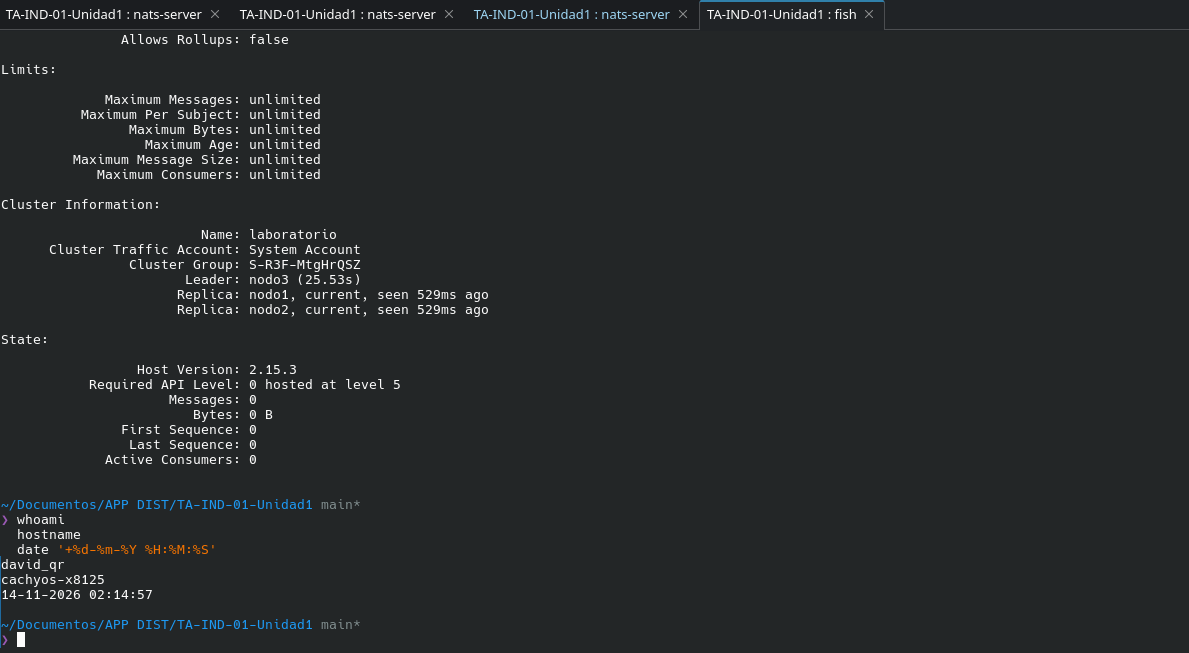
\includegraphics[width=0.97\linewidth,height=0.29\textheight,keepaspectratio]{03_cluster_replicado.png}
\caption{Flujo replicado: nodo3 es líder, nodo1 y nodo2 están sincronizados. Captura propia del 14-11-2026.}
\label{fig:replicas}
\end{figure}
\begin{figure}[H]
\centering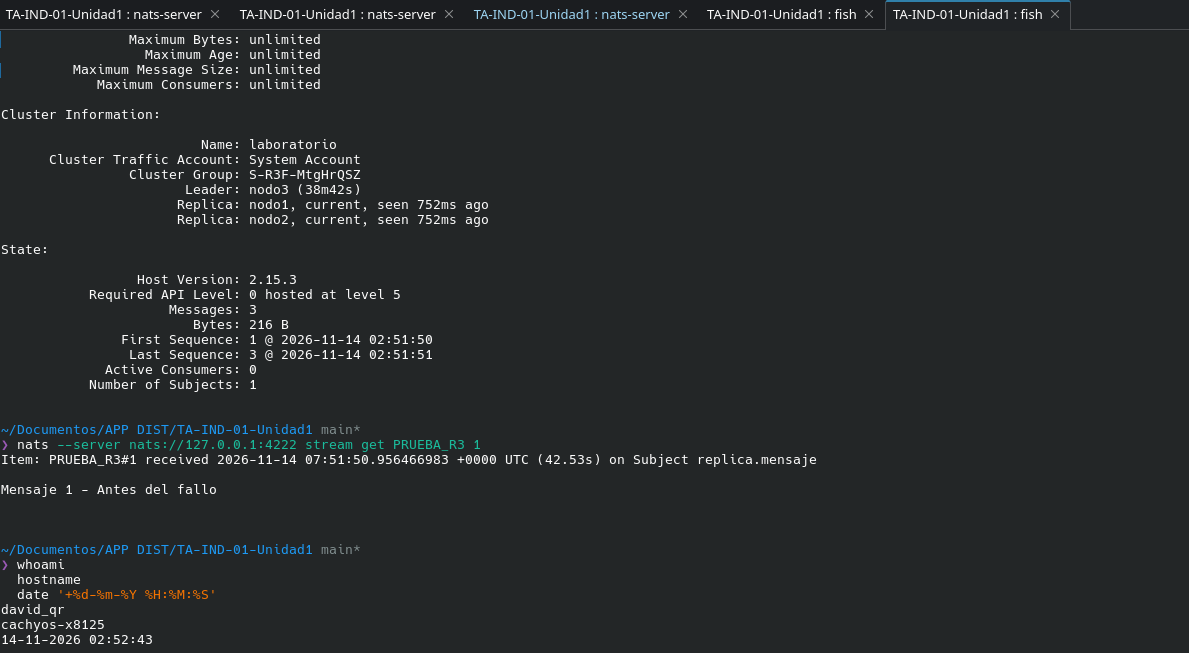
\includegraphics[width=0.97\linewidth,height=0.29\textheight,keepaspectratio]{04_mensajes_antes_fallo.png}
\caption{Tres mensajes almacenados y recuperación del primero antes de interrumpir el líder.}
\label{fig:antesfallo}
\end{figure}
\begin{figure}[H]
\centering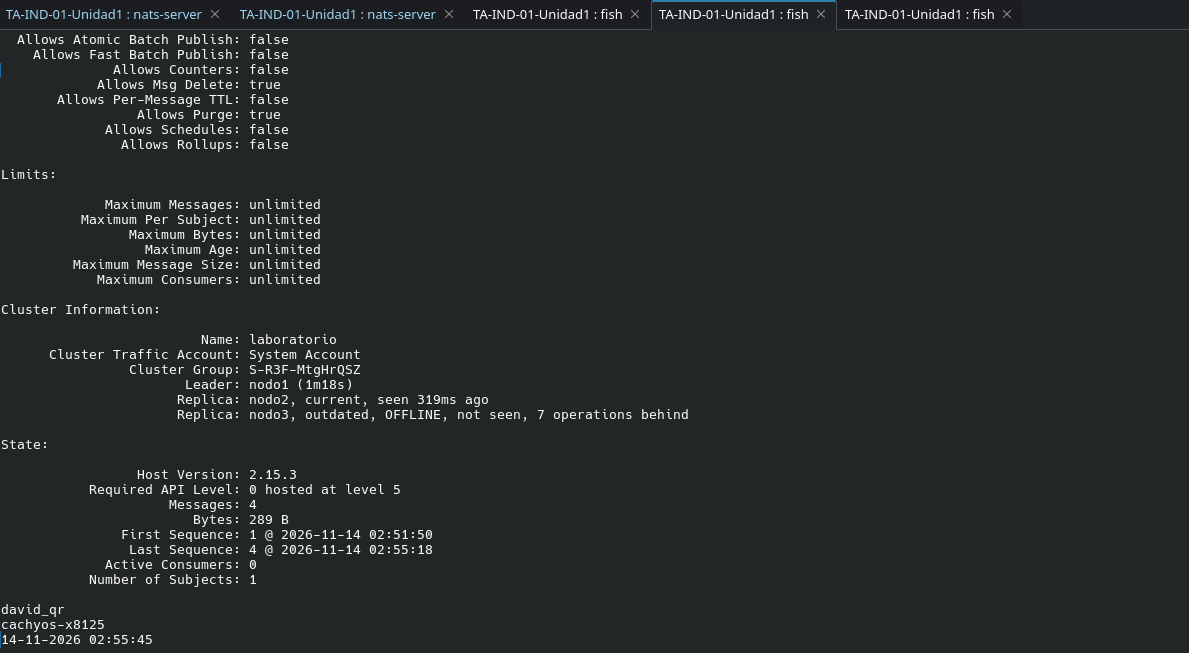
\includegraphics[width=0.97\linewidth,height=0.29\textheight,keepaspectratio]{05_caida_nodo_lider.png}
\caption{Tras detener nodo3: nodo1 lidera, nodo3 aparece desconectado y el flujo contiene cuatro mensajes.}
\label{fig:durantefallo}
\end{figure}
\begin{figure}[H]
\centering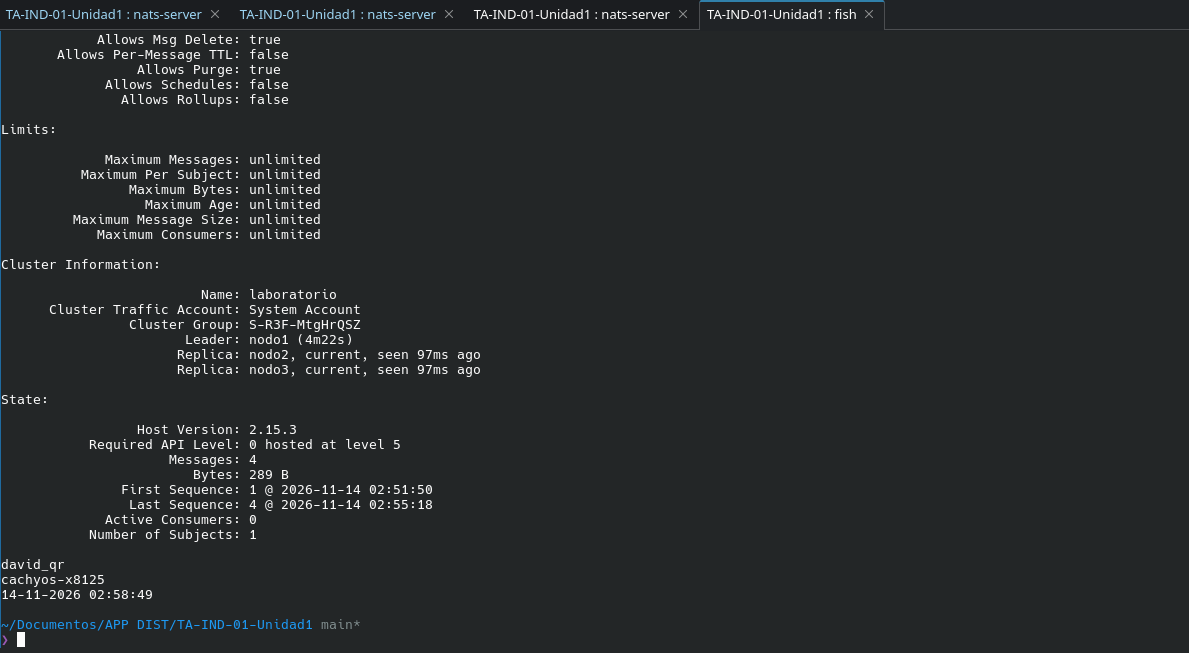
\includegraphics[width=0.97\linewidth,height=0.29\textheight,keepaspectratio]{06_recuperacion_nodo.png}
\caption{Recuperación: nodo3 vuelve a estar actualizado y se conservan los cuatro mensajes.}
\label{fig:recuperacion}
\end{figure}

La evidencia respalda que el flujo siguió respondiendo a lecturas y almacenó un nuevo mensaje mientras quedaban disponibles dos de las tres réplicas. Es coherente con el mecanismo de mayoría de Raft explicado por NATS \cite{natsreplication}. No se obtuvieron métricas de latencia, no se perdió el quórum y no se simuló una partición de red. El informe, por tanto, no generaliza esta observación a cualquier escenario de fallo ni la presenta como prueba experimental de CAP o PACELC.

\section{Ejemplos del entorno del estudiante}
Las experiencias con aplicaciones cotidianas permiten reconocer la latencia y la concurrencia desde el lado del usuario. No obstante, el comportamiento de una interfaz no revela por sí solo la arquitectura, los algoritmos de consenso ni la causa concreta de una falla.

\subsection{Jóvenes en Acción: lentitud durante una demanda elevada}
Al utilizar la plataforma Jóvenes en Acción, experimenté una lentitud excesiva: las páginas tardaban en responder y prácticamente no se podían realizar las operaciones previstas. La situación coincidía con un período de alta demanda de acceso, por lo que el número de solicitudes simultáneas parecía influir en el rendimiento. Desde mi experiencia observé una pérdida de capacidad de respuesta, no la causa exacta del problema.

El caso se relaciona con la \textbf{concurrencia}, porque muchos usuarios pueden solicitar recursos al mismo tiempo; con la \textbf{latencia}, por el retraso visible en las respuestas; y con la \textbf{escalabilidad}, por la necesidad de sostener el servicio cuando aumenta la carga. Sin registros del servidor, mediciones de tráfico ni detalles de su infraestructura, no se puede asegurar que el problema se debiera exclusivamente a solicitudes concurrentes o a un fallo distribuido.

\subsection{WhatsApp: demora entre dos dispositivos cercanos}
En otra ocasión envié un mensaje por WhatsApp a un amigo que estaba a mi lado. Ambos teléfonos estaban conectados a la misma red Wi-Fi, pero el mensaje tardó en llegar, como si alguno de los dispositivos no tuviera conexión. La cercanía física y la red compartida no evitaron el retraso observado.

Esta situación ilustra la \textbf{latencia de entrega} y la \textbf{comunicación asíncrona}: el emisor puede enviar un mensaje y el receptor recibirlo más tarde, sin que ambos procesos deban ocurrir simultáneamente. No conocemos la ruta exacta que siguió el mensaje ni qué componente produjo la demora; podría depender de la conexión, el servicio o los propios dispositivos. Por ello, el ejemplo describe una observación de usuario y no una prueba de fallos o replicación en los servidores de WhatsApp.

\section{Análisis comparativo: NATS JetStream frente a Apache Pulsar}
Ambos sistemas permiten intercambiar mensajes y conservarlos para procesamiento posterior, pero organizan de manera distinta el almacenamiento y la coordinación. La tabla compara las arquitecturas y garantías documentadas, no cifras medidas directamente entre los productos: Apache Pulsar no se ejecutó en el laboratorio. La documentación de Pulsar describe brokers que atienden clientes, un almacén de metadatos y un conjunto de servidores BookKeeper (\emph{bookies}) que guardan los registros persistentes \cite{pulsararchitecture}. En JetStream, los propios servidores NATS pueden almacenar las réplicas de un flujo y coordinarse mediante Raft \cite{natsclustering,natsreplication}.

\begingroup\small
\begin{longtable}{@{}p{3.05cm}p{5.25cm}p{5.25cm}@{}}
\caption{Comparación de decisiones de diseño entre JetStream y Pulsar.}\label{tab:comparacion}\\
\toprule
\textbf{Criterio} & \textbf{NATS JetStream} & \textbf{Apache Pulsar} \\\midrule
\endfirsthead
\toprule
\textbf{Criterio} & \textbf{NATS JetStream} & \textbf{Apache Pulsar} \\\midrule
\endhead
Arquitectura & Servidores NATS interconectados; los nodos con JetStream almacenan réplicas del flujo. & Brokers de atención a clientes, servicio de metadatos y almacenamiento persistente distribuido en BookKeeper. \\
Modelo de comunicación & Cliente--servidor y publicación/suscripción; almacenamiento y recuperación con JetStream. & Cliente--broker y publicación/suscripción con temas y suscripciones. \\
Replicación & Réplicas del flujo coordinadas por Raft; en \(R=3\) se requiere mayoría de dos. & Réplicas de entradas de los ledgers en los \emph{bookies}, con parámetros de escritura y confirmación configurables. \\
Tolerancia a fallos & Con mayoría disponible puede elegir nuevo líder y continuar escrituras confirmadas. & Se recuperan ledgers y propiedad de temas ante fallos; depende de brokers, metadatos y quórum de BookKeeper. \\
Transparencia de ubicación & El acceso al flujo oculta en parte qué nodo mantiene su líder; los clientes deben disponer de servidores accesibles. & El descubrimiento de servicios y la redirección permiten localizar el broker propietario de cada tema. \\
Consistencia y CAP & La confirmación de escritura replicada necesita quórum; una minoría aislada no puede confirmar nuevas escrituras. & Las garantías de cada ledger dependen de BookKeeper y de la configuración de sus quórums; no procede imponerle una etiqueta CAP única. \\
Escalamiento y operación & En el laboratorio de tres procesos fue sencillo desplegarlo y observarlo; el costo crece con réplicas y operaciones. & Se pueden escalar por separado los brokers y el almacenamiento, con más componentes administrativos. \\
Aplicaciones ilustradas & Bus de eventos entre clústeres en una plataforma IoT documentada por Ju y colaboradores \cite{ju2026}. & Canalizaciones de datos con multitenencia y geo-replicación descritas por Do y colaboradores \cite{do2025}. \\
\bottomrule
\end{longtable}
\endgroup

La diferencia más clara es la separación de responsabilidades. En NATS JetStream, tres procesos bastaron para reproducir un flujo con replicación y fallo controlado. En Pulsar, la separación de \emph{brokers} y \emph{bookies} facilita crecer de forma independiente en capacidad de atención y de almacenamiento, pero supone configurar y operar más piezas. Esto no convierte automáticamente al primero en ``más rápido'' ni al segundo en ``más seguro'': esas conclusiones requerirían una prueba comparable en condiciones controladas. Dyjach y Plechawska-Wójcik observaron resultados favorables a Pulsar en determinados escenarios frente a Kafka y RabbitMQ; no compararon Pulsar con JetStream, así que esas mediciones solo proporcionan contexto sobre cargas y rendimiento \cite{dyjach2024}.

\section{Postura crítica y compromisos de diseño}
Para una aplicación pequeña o un laboratorio, la posibilidad de configurar tres servidores NATS y comprobar directamente un cambio de líder es una ventaja de JetStream. La abstracción de \emph{subjects} y \emph{streams} permite separar al productor del lector y agregar persistencia sin desarrollar una infraestructura propia de almacenamiento distribuido. La prueba realizada confirma esa utilidad en un entorno local reducido \cite{natsjetstream}.

La disponibilidad lograda tiene condiciones: dos de las tres réplicas deben poder comunicarse y no basta con que los procesos continúen abiertos. Con pérdida de la mayoría, la confirmación de escrituras no puede continuar normalmente, ya que el consenso impide que dos grupos aislados se consideren líderes válidos del mismo flujo. Esta es una limitación deliberada para proteger la coherencia del registro replicado, no una falla accidental de configuración \cite{natsreplication}.

La replicación tampoco sustituye las copias de seguridad, el monitoreo ni la planificación ante pérdida del equipo completo. En el experimento los tres nodos compartían CachyOS, su almacenamiento físico y su alimentación eléctrica; por eso el sistema podía tolerar una caída de proceso, pero no estaba protegido frente a una interrupción total del equipo. Tampoco se hizo una medición sistemática de rendimiento, por lo que sería incorrecto afirmar una ventaja de latencia respecto de Pulsar.

En un servicio que requiera escalar de manera independiente grandes volúmenes de datos y el tráfico atendido por los brokers, la arquitectura con BookKeeper de Pulsar podría ser preferible. A cambio, requiere administrar capas de almacenamiento, metadatos y corredores, cuyo estado y configuración influyen en la recuperación. Los artículos científicos consultados respaldan usos y características específicas, pero no permiten decidir un ganador general para todas las cargas \cite{pulsararchitecture,do2025,dyjach2024}.

El reporte público sobre pruebas con particiones y cambios de membresía en NATS también recuerda que no basta un único ensayo exitoso para validar escenarios extremos \cite{natsincident2025}. Antes de recomendar JetStream para información crítica harían falta pruebas de fallos múltiples, cortes abruptos, políticas de persistencia, duplicados, reintentos y restauración, además de comprobar el comportamiento con versiones concretas del producto. Esas pruebas quedan fuera del alcance de esta actividad.

\section{Conclusiones}
El clúster de tres nodos con \texttt{PRUEBA\_R3} permitió observar el cambio de liderazgo después de detener \texttt{nodo3}: \texttt{nodo1} asumió el rol y el flujo conservó los tres mensajes previos y almacenó un cuarto. La reincorporación de \texttt{nodo3} terminó con las dos réplicas seguidoras en estado \texttt{current}. Estos hechos respaldan la tolerancia a un fallo de proceso mientras se conserva un quórum de dos nodos en este montaje específico.

La interpretación depende del tipo de evidencia. Las capturas confirman la continuidad del flujo y la recuperación del nodo, pero no prueban el comportamiento bajo particiones ni permiten estimar la latencia de las confirmaciones. Para esos aspectos se emplearon la documentación de Raft y los límites de consistencia descritos por NATS, evitando convertir supuestos técnicos en mediciones inexistentes.

La comparación con Apache Pulsar muestra dos formas distintas de organizar la persistencia: JetStream replica flujos entre servidores NATS, mientras Pulsar separa el servicio de mensajes del almacenamiento BookKeeper. Ninguna de las dos arquitecturas es universalmente superior; su conveniencia depende del volumen de datos, la administración disponible y las garantías que requiera la aplicación. La principal lección del ensayo es que la replicación mejora la continuidad frente a fallos concretos, pero su alcance siempre debe explicarse junto con las condiciones del experimento.

\section*{Declaración de uso de inteligencia artificial}
\addcontentsline{toc}{section}{Declaración de uso de inteligencia artificial}
Se utilizó ChatGPT (GPT-6) como apoyo para organizar la estructura, elaborar borradores de varias secciones, preparar una plantilla editable del diagrama y revisar la redacción y los datos bibliográficos. Las pruebas, las capturas y los resultados experimentales se obtuvieron en el equipo del estudiante. El análisis se contrastó con los artículos consultados, la documentación técnica y las evidencias del repositorio; los ejemplos del entorno proceden de experiencias comunicadas por el estudiante.

\printbibliography[title={Referencias}]

\appendix
\section{Anexo A: Esquema inicial a mano}
\IfFileExists{../Anexos/esquema_inicial.jpeg}{%
\begin{figure}[H]\centering
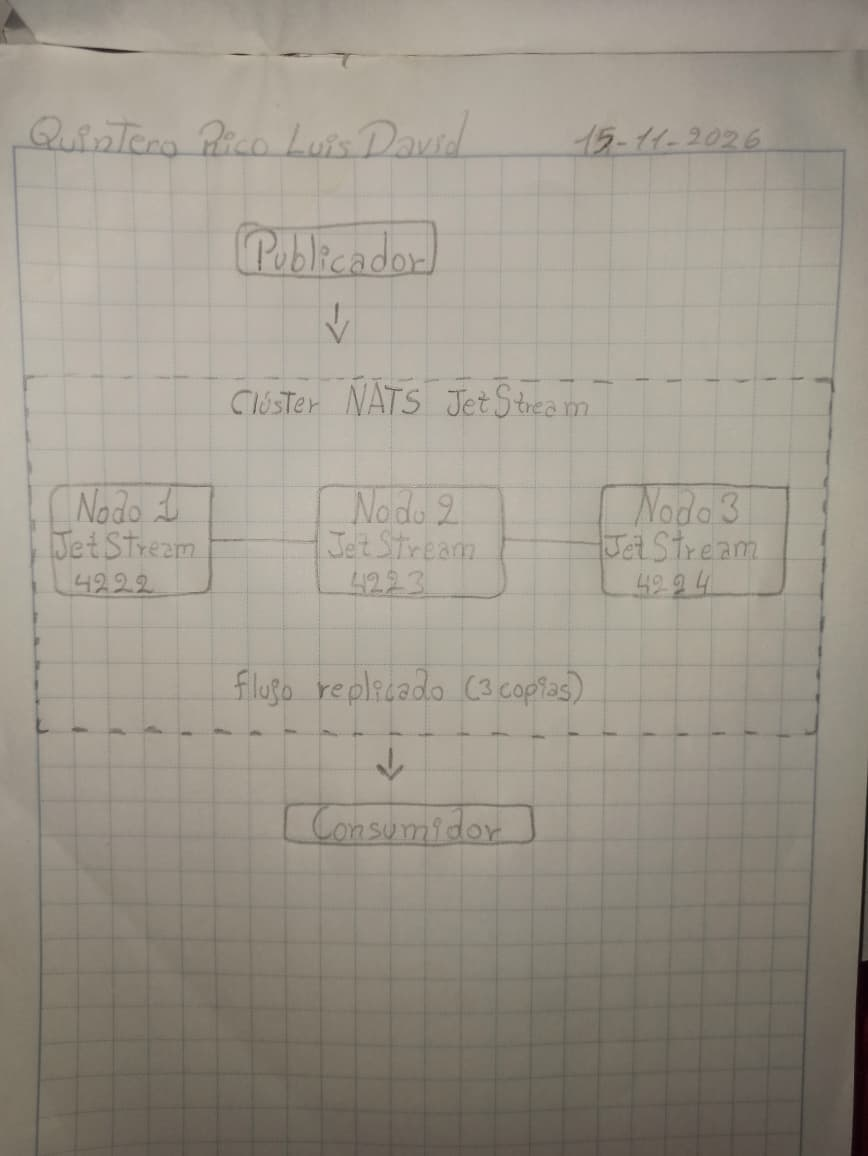
\includegraphics[height=0.67\textheight,keepaspectratio]{esquema_inicial.jpeg}
\caption{Bosquejo a mano. La fecha de la hoja corresponde a su presentación o finalización.}
\end{figure}
}{%
\IfFileExists{../anexos/esquema_inicial.jpeg}{%
\begin{figure}[H]\centering
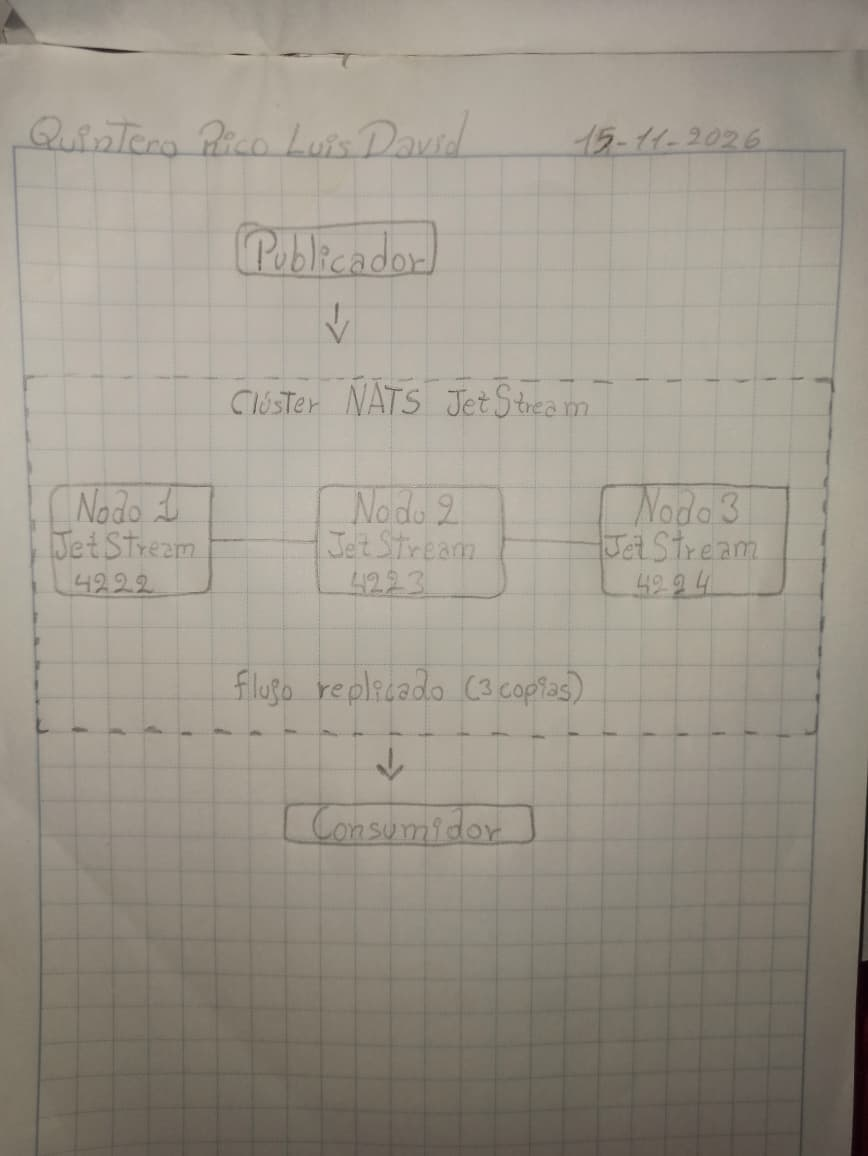
\includegraphics[height=0.67\textheight,keepaspectratio]{esquema_inicial.jpeg}
\caption{Bosquejo a mano. La fecha de la hoja corresponde a su presentación o finalización.}
\end{figure}
}{\PackageError{TA-IND-01}{Falta la fotografia del Anexo A}{Guarde esquema_inicial.jpeg en Anexos/ o anexos/.}}}

\section{Anexo B: Capturas de lectura de fuentes}
\begin{figure}[H]
\centering
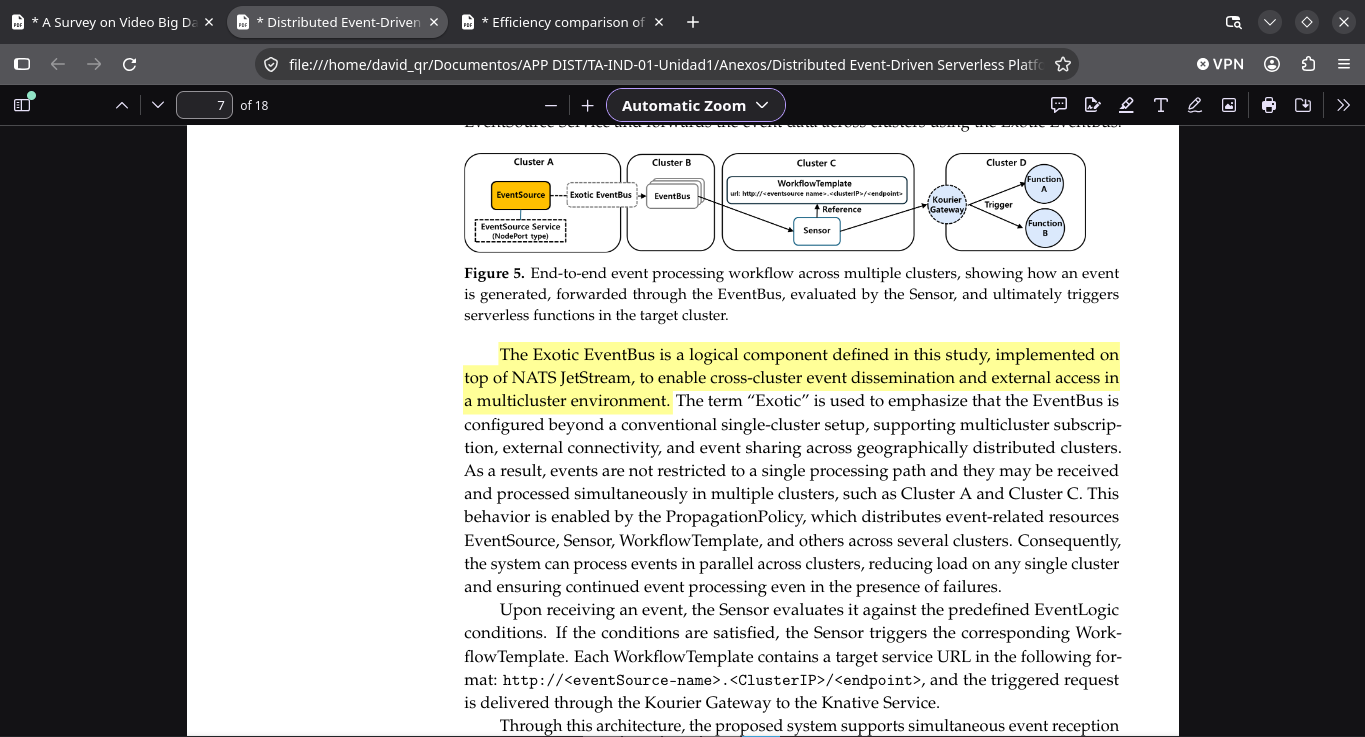
\includegraphics[width=0.96\linewidth,keepaspectratio]{01_nats_jetstream.png}
\caption{Ju, Seo y Kim (2026), p. 7: bus de eventos basado en JetStream. El fragmento corresponde a \cite{ju2026}.}
\end{figure}

\begin{figure}[H]
\centering
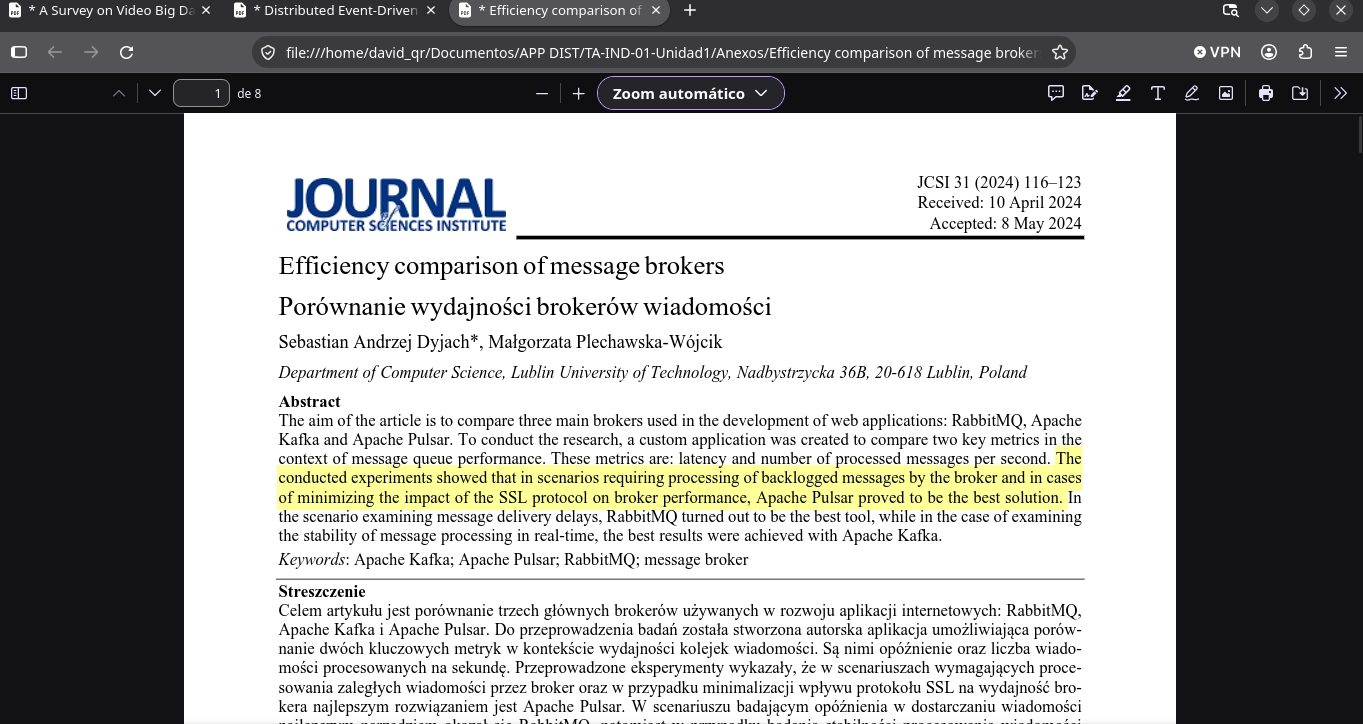
\includegraphics[width=0.96\linewidth,keepaspectratio]{02_pulsar_rendimiento.png}
\caption{Dyjach y Plechawska-Wójcik (2024), p. 116: resultados de rendimiento en Pulsar. Véase \cite{dyjach2024}.}
\end{figure}

\begin{figure}[H]
\centering
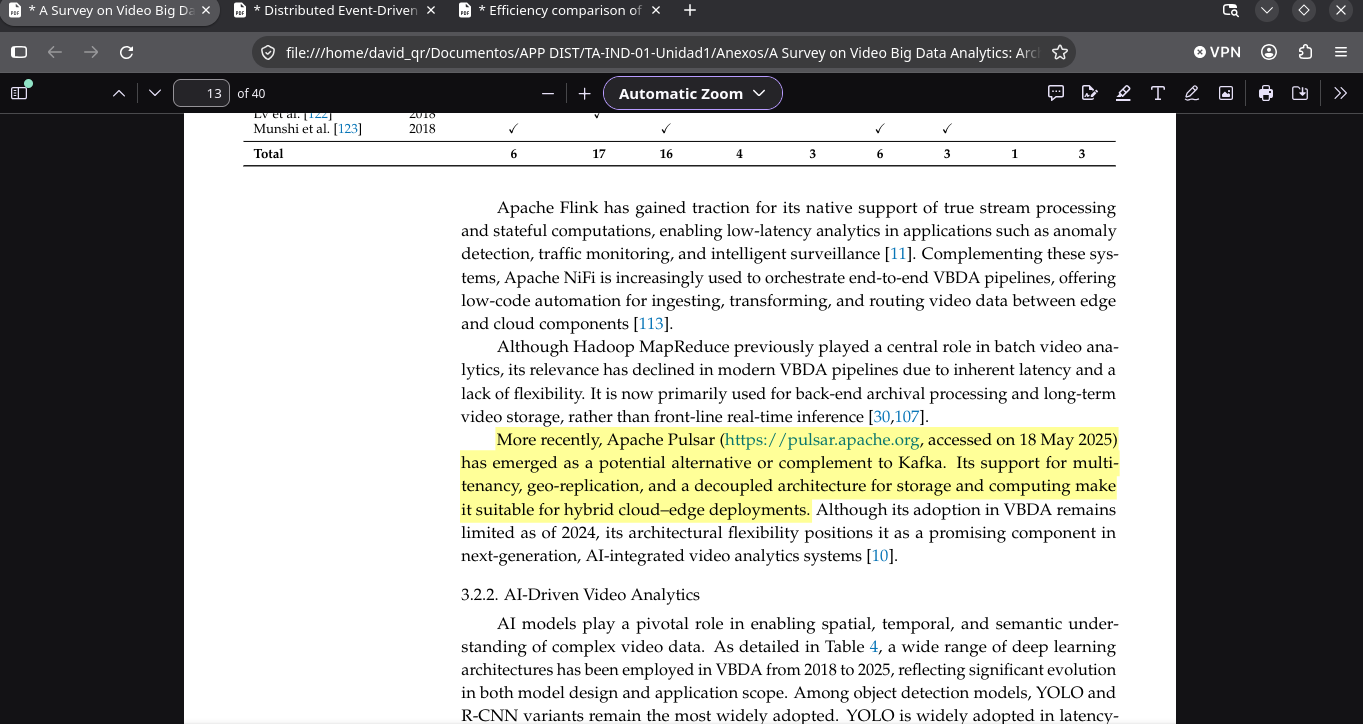
\includegraphics[width=0.96\linewidth,keepaspectratio]{03_pulsar_arquitectura.png}
\caption{Do y colaboradores (2025), p. 13: propiedades arquitectónicas de Pulsar. Véase \cite{do2025}.}
\end{figure}

\end{document}
